\documentclass{beamer}
\usepackage{pgfpages}
\setbeameroption{show notes on second screen}

\setbeamertemplate{navigation symbols}{}%remove navigation symbols
\setbeamertemplate{footline}[frame number]
\mode<presentation>{}

\usepackage{tikz}
\usetikzlibrary{calc,shapes.multipart,chains,arrows,matrix,fit}
\usepackage{listings}
\usepackage{algpseudocode}
\usepackage{array}

%% preamble
\title{Enhancements to Looping Constructs Using Prefetching and Exploiting GPU}
\author{Anurag Peshne}
\date{15 May 2018}

\begin{document}
%% title frame
\begin{frame}
  \titlepage
\end{frame}

%% normal frame
\begin{frame}\frametitle{Contents}
  \note[item]{Agenda for today.}
  \pause
  \begin{itemize}
    \note[item]{First some background, what is SIA, how it works.}
  \item Super Instruction Architecture (SIA)
    \pause
    \note[item]{What we did.}
  \item 2 Enhancements
    \pause
    \begin{itemize}
    \item Prefetching
      \pause
    \item Exploiting GPU
      \pause
    \end{itemize}
    \note[item]{The experiments carried out to evaluate the work}
  \item Experiments
    \pause
  \item Conclusion
    \note[item]{And finally, the conclusions}
  \end{itemize}
\end{frame}

\begin{frame}[fragile]\frametitle{SIA}
  \begin{itemize}
    \pause
  \item Parallel Programming Environment.
    \pause
  \item Engineered to solve very large computation problems expressed in terms of
    operation on multidimensional arrays.
    \pause
  \item Algorithms are expressed in terms of blocks or multidimensional arrays
    rather than individual floating point numbers:
    \begin{lstlisting}[]
      do i
        do j
          x = A[i,j] * B[i,j]
        enddo j
      enddo i
    \end{lstlisting}
    \note[item]{It is more efficient to move numbers in blocks rather than individual
      blocks}
    \note[item]{Runtime can also schedule other things while transfering is in progress}
    \pause
  \item \textit{Super} Instructions acting upon \textit{Super} Numbers.
    \note[item]{Super Instructions work on block, looping on block handled automatically}
    \note[item]{This also relieves programmer from error prone index calculation}
  \end{itemize}
\end{frame}

\begin{frame}\frametitle{SIA}
  \begin{itemize}
    \pause
  \item SIMD: can execute instructions in parallel over multiple processors.
    \note[item]{Blocks of same array distributed on different workers}
    \pause
  \item Can be deployed and scaled on multiple nodes in high performance computing cluster.
    \pause
  \item Can support arrays larger than combined memory of all nodes in cluster by
    swapping chunks that are not \textit{hot} on hard drive.
    \pause
  \item Participating nodes in cluster are divided into Servers and Workers:
    \begin{itemize}
      \pause
    \item Servers deal with swapping the blocks and serving the request for blocks
      by workers.
      \pause
    \item Workers do the actual computation.
      \note[item]{They request for specific block when needed.}
    \end{itemize}
    \pause
  \item SIA consists of:
    \begin{itemize}
      \pause
    \item Super Instruction Assembly Language (SIAL)
      \pause
    \item SIA Runtime
    \end{itemize}
  \end{itemize}
\end{frame}

\begin{frame}\frametitle{SIAL}
  \begin{itemize}
    \pause
  \item Domain Specific Language
    \note[item]{Separation of concern: domain programmer deal with domain logic,
      runtime handles scheduling, executing in parallel, choosing optimization etc}
    \pause
  \item Support for Blocks as first class citizen.
    \pause
  \item Intended to be used by domain programmer.
    \note[item]{High level, easy for domain programmer to code using it.}
    \pause
  \item Dynamically Interpreted.
    \note[item]{Interpreter can do tricks like executing on GPU if available or falling back to CPU if not}
    \pause
  \item \texttt{do} and \texttt{pardo}
    \pause
  \item Super Instructions can be defined using C, C++, Fortran
    \pause
    or CUDA.
    \note[item]{Programmer can define customized super instruction which are domain
      specific}
    \note[item]{easy to port to CUDA}
  \end{itemize}
\end{frame}

\begin{frame}\frametitle{Looping Constructs}
  \begin{itemize}
  \item \texttt{do}, \texttt{pardo}
    \note[item]{One of the most important constructs in language}
    \pause
  \item 2 Enhancements:
    \begin{itemize}
    \item Prefetching
    \item Exploiting GPU
    \end{itemize}
  \end{itemize}
\end{frame}

\begin{frame}[label=prefetchcode]\frametitle{Prefetching}
%\hline
\begin{algorithmic}[1]
%\caption{An example of typical workflow in SIAL}
\Loop
\State $GET\ A[i, j]$\Comment{Non Blocking}
\State $GET\ B[j, k]$
\State $t\_result[j, k] \gets A[i, j] \times B[j, k]$\Comment{Compute bound}
\State $CALL\ compute\_fun(t\_result[j, k])$
\State $PUT\ AB[i, k] \gets t\_result[i, k]$\Comment{Blocking Network bound}
\EndLoop
%\hline
\end{algorithmic}
\note[item]{Blocks at line 4: contraction.}
\note[item]{Compute resources wasted during network transfer, same in last line.
  PUT is blocking}
\note[item]{Network resources wasted during computing}
% Notes for 2 occurrence of this slide
\note[item]{------------------------------------------------------------------}
\note[item]{So for example, here \texttt{GET} on line 2 can prefetch independently
  of \texttt{GET} on line 3.}
\end{frame}

\begin{frame}\frametitle{Prefetching}
  \begin{itemize}
  \item Similar to h/w prefetching:
    \note[item]{Explain h/w prefetching: how processor prefetches block of memory
      in anticipation that it will be needed}
    \begin{itemize}
      \pause
    \item Moving from slower memory to faster memory.
      \note[item]{RAM to cache memory; SIA: server memory to local client memory}
      \pause
    \item Need to guess what to prefetch \pause and how much to prefetch.
    \end{itemize}

    \pause
  \item Not exactly similar:
    \begin{itemize}
    \item In h/w there is anticipation, in SIA we \textit{know} precisely what to
      prefetch.
      \pause
    \item We know when to evict from cache.
      \note[item]{h/w may keep some blocks in memory in anticipation that it might
        be needed again}
    \end{itemize}
  \end{itemize}
\end{frame}

\begin{frame}\frametitle{Prefetching Implementation}
  \begin{itemize}
  \item Before prefetching:
    \begin{itemize}
    \item Get values of indices
    \item increment according to the loop
    \item Update values of indices
    \end{itemize}
  \end{itemize}
\end{frame}

\begin{frame}[fragile]\frametitle{Prefetching Implementation}
\begin{figure}
  \centering

  \tikzstyle{table}=[
  matrix of nodes,
  row sep=-\pgflinewidth,
  column sep=-\pgflinewidth,
  nodes={rectangle,draw=black,text width=12ex,align=center},
  text depth=0.25ex,
  text height=1.5ex,
  nodes in empty cells]
  \begin{tikzpicture}[list/.style={rectangle split, rectangle split parts=6,
      draw, rectangle split horizontal}, >=stealth, start chain]

    \node[list,on chain] (A) {};
    \note[item]{Here we first calculate the set of indices}
    \pause
    \node[list,on chain] (B) {};
    \note[item]{Then calculate next set using previous set, before actually iterating over the loop}
    \pause
    \node[list,on chain] (C) {};
    \note[item]{And so on...}
    \pause
    \node[on chain,draw,inner sep=6pt] (D) {};
    \draw (D.north east) -- (D.south west);
    \draw (D.north west) -- (D.south east);
    \draw[*->] let \p1 = (A.six), \p2 = (A.center) in (\x1,\y2) -- (B);
    \draw[*->] let \p1 = (B.six), \p2 = (B.center) in (\x1,\y2) -- (C);
    \draw[*->] let \p1 = (C.six), \p2 = (C.center) in (\x1,\y2) -- (D);

    \note[item]{Creating list of indices}
    \pause
    \matrix (map) [table,below=of A]
    {
      LineNumber & Reference  \\
      101        &            \\
      102        &            \\
      \vdots     & \vdots     \\
    };

    \note[item]{Save which set of indices is prefetched by each \texttt{GET} in the loop}
    \pause
    \draw[*->] (map-2-2.center) to[out=0, in=270] (B.south);
    \pause
    \draw[*->] (map-3-2.center) to[out=0, in=270] (C.south);
  \end{tikzpicture}
\end{figure}
\end{frame}

\againframe{prefetchcode}

\begin{frame}\frametitle{Prefetching Mechanism}
  \begin{itemize}
  \item Function \texttt{update\_indices} divided into 3 functions:
    \begin{itemize}
      \pause
    \item \texttt{peek\_indices}
      \note[item]{returns set of indices, internally taking care of maintaining
        and generating next indices lazily if required}
      \pause
    \item \texttt{prefetch\_indices}
      \note[item]{remembers the state of each \texttt{GET} and automatically returns
        next set of indices for each \texttt{GET}}
      \pause
    \item \texttt{update}
      \note[item]{pops the first element in the list and updates the interpreter
        state}
    \end{itemize}
  \end{itemize}
\end{frame}

\begin{frame}\frametitle{Prefetching Mechanism}
  \begin{figure}[h] %place figure "here"
    \centering
    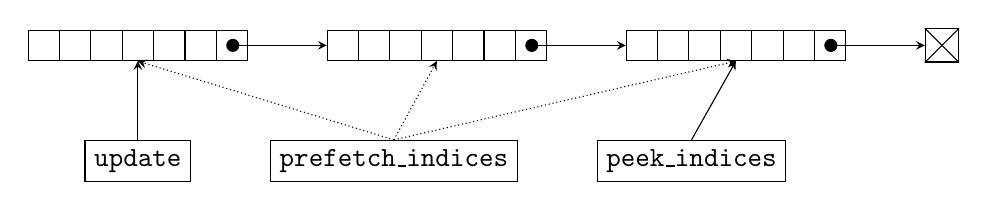
\begin{tikzpicture}[
      list/.style={rectangle split, rectangle split parts=7,
        draw, rectangle split horizontal},
      function/.style={rectangle, draw,align=center},
      >=stealth, start chain]

      \node[list,on chain] (A) {};
      \node[list,on chain] (B) {};
      \node[list,on chain] (C) {};
      \node[on chain,draw,inner sep=6pt] (D) {};
      \draw (D.north east) -- (D.south west);
      \draw (D.north west) -- (D.south east);
      \draw[*->] let \p1 = (A.seven), \p2 = (A.center) in (\x1,\y2) -- (B);
      \draw[*->] let \p1 = (B.seven), \p2 = (B.center) in (\x1,\y2) -- (C);
      \draw[*->] let \p1 = (C.seven), \p2 = (C.center) in (\x1,\y2) -- (D);

      \note[item]{We have same list from last time}
      \pause
      \node[function, below=of A]        (update)   {\texttt{update}};
      \node[function, right=of update]   (prefetch) {\texttt{prefetch\_indices}};
      \node[function, right=of prefetch] (peek)     {\texttt{peek\_indices}};

      \draw[->]                (update.north)   -- (A.south);
      \draw[densely dotted,->] (prefetch.north) -- (A.south);
      \draw[densely dotted,->] (prefetch.north) -- (B.south);
      \draw[densely dotted,->] (prefetch.north) -- (C.south);
      \draw[->]                (peek.north)     -- (C.south);

      \note[item]{\texttt{peek\_indices} produced, \texttt{prefetch\_indices} is
        free to roam along the list, \texttt{update} consumes a set of indices from
        the list.}
    \end{tikzpicture}
  \end{figure}
\end{frame}

\begin{frame}\frametitle{Hit Ratio}
  \note[item]{To study the effectiveness of the prefetching, \texttt{hit\_ratio},
    another metric is introduced.}
  \pause
  \[
    \texttt{hit\_ratio} = \frac{number~of~times~no~blocking~required}{total~number~of~times~data~accessed}
  \]
  \note[item]{The \texttt{hit\_ratio} represents the number of times prefetching
    was successful to hide network transfer cost.}
\end{frame}

\begin{frame}\frametitle{Prefetching Experiments: Index Length}
  \note[item]{Index length is the length of range of indices: when looping on
    \texttt{i}, it goes from 2 to 5 or 2 to 10}
  \pause
  \begin{figure}[h]
    \resizebox{.9\linewidth}{!}{\input{results/index_length/hitratio}}
    \caption{Index Range Length v/s \texttt{hit\_ratio}}
  \end{figure}
  \note[item]{Several things to note: the lowest hit ratio is 0.65, because...}
  \note[item]{as the lenght of range of indices increase, the prefetching kicks in}
  \note[item]{eventually flattens out}
\end{frame}

\begin{frame}\frametitle{Prefetching Experiments: First Iteration}
  \note[item]{Side effect of prefetching: with prefetching, the first request becomes
    heavy}
  \pause
  \begin{figure}[h]
    \resizebox{.9\linewidth}{!}{\input{results/index_length/p_first_mean}}
    \caption{Index Range v/s \texttt{wait\_time\_} per iteration}
  \end{figure}
  \note[item]{As prefetching kicks in, the first request becomes costlier}
  \note[item]{note mean is reducing}
  \note[item]{looking other way round, prefetching is kicking in}
\end{frame}

\begin{frame}\frametitle{Prefetching Experiments: Mean}
  \note[item]{Overall wait time by \texttt{GET}}
  \pause
  \begin{figure}[h]
    \resizebox{.9\linewidth}{!}{\input{results/index_length/p_np_mean}}
    \caption{Index Range v/s \texttt{wait\_time\_} per iteration in Prefetched and no Prefetched Loop}
  \end{figure}
  \note[item]{Prefetching helps!}
\end{frame}

\begin{frame}\frametitle{Prefetching Experiments: Block Size First Iteration}
  \note[item]{How block size affects first iteration}
  \pause
  \begin{figure}[h]
    \resizebox{.9\linewidth}{!}{\input{results/block_size/first_wait_time}}
    \caption{Block Size v/s \texttt{wait\_time\_} for first iteration}
  \end{figure}
  \note[item]{block size affects first iteration}
\end{frame}

\begin{frame}\frametitle{Prefetching Experiments: Block Size Mean}
  \note[item]{How block size affects overall time}
  \pause
  \begin{figure}[h]
    \resizebox{.9\linewidth}{!}{\input{results/block_size/avg_wait_time}}
    \caption{Block Size v/s Mean \texttt{wait\_time\_} for Prefetched and No Prefetch Loop}
  \end{figure}
  \note[item]{Prefetching is paying off, 'Prefetch' time not so much affected}
\end{frame}

\begin{frame}\frametitle{Prefetching: Putting it all together}
  \note[item]{Just to look at whole picture}
  \pause
  \begin{figure}[h]
    \resizebox{.9\linewidth}{!}{\input{results/block_size/avg_all}}
    \caption{Block Size v/s Mean \texttt{wait\_time\_} for Prefetched and No Prefetch Loop}
  \end{figure}
\end{frame}

\begin{frame}\frametitle{Prefetching: Number of Blocks to Prefetch}
  \note[item]{\texttt{wait\_time} for the \textbf{first} iteration}
  \pause
  \begin{figure}[h]
    \resizebox{.9\linewidth}{!}{\input{results/look_ahead/first_wait_time}}
    \caption{Number of Block Prefetched v/s \texttt{wait\_time\_} for first request}
  \end{figure}

  \note[item]{\texttt{wait\_time\_} for the first request grows linearly with the
    number of blocks to prefetch}
  \note[item]{Thus the number of blocks to prefetch cannot be set at very high
    number unless the length of index range is known to be large}
\end{frame}

\begin{frame}\frametitle{Prefetching: Number of Blocks to Prefetch}
  \note[item]{This time to overall mean \texttt{wait\_time}}
  \pause
  \begin{figure}[h]
    \resizebox{.9\linewidth}{!}{\input{results/look_ahead/avg_wait_time}}
    \caption{Number of Block Prefetched v/s mean \texttt{wait\_time\_}}
  \end{figure}
  \note[item]{First sharp decrease as prefetching kicks in then increase due to
    costly first iteration}
\end{frame}

\begin{frame}\frametitle{Prefetching: Number of Blocks to Prefetch}
  \note[item]{now lets look at this number v/s hit ratio}
  \pause
  \begin{figure}[h]
    \resizebox{.9\linewidth}{!}{\input{results/look_ahead/hit_ratio}}
    \caption{Number of Block Prefetched v/s Hit Ratio for first request}
  \end{figure}
  \note[item]{Hit ratio saturates after hitting a critical amount. There is no
    much use after that to increase number of blocks to prefetch.}
  \note[item]{This explains the rise in mean \texttt{wait\_time\_} as
    \texttt{wait\_time\_} for first request grows and the number of blocks
    available without blocking stays constant.}
\end{frame}

\begin{frame}[fragile=singleslide]\frametitle{Exploiting GPU: ACESIII}
\begin{lstlisting}
gpu_begin
gpu_put aoint(lambda,mu,sigma,nu) #allocate & copy
DO j1
    gpu_put LT2AOab1(mu,i1,nu,j1)
    ...
ENDDO j1
...
DO j
    gpu_allocate Yab(mu,i,nu,j) # allocate temp
    Yab(mu,i,nu,j) = aoint(lambda,mu,sigma,nu)*LTAOab(lambda,i,sigma,j)
    gpu_free Yab(mu,i,nu,j) #free
    ...
    gpu_get LT2AOab1(mu,i1,nu,j1)
    gpu_free LTAOab(lambda,i1,sigma,j1)
    ...
gpu_free aoint(lambda,mu,sigma,nu)
gpu_end
\end{lstlisting}
\note[item]{mark GPU region}
\note[item]{allocate memory on GPU and copy CPU to GPU}
\note[item]{free memory on GPU}
\end{frame}

\begin{frame}[fragile]\frametitle{Automatic GPU Memory Synchronization}
  \pause
\begin{figure}[h] %place figure "here"
  \centering

  \tikzstyle{table}=[
  matrix of nodes,
  row sep=-\pgflinewidth,
  column sep=-\pgflinewidth,
  nodes={typetag}]
  \begin{tikzpicture}[list/.style={rectangle split, rectangle split parts=3,
      draw, rectangle split horizontal,align=center}, >=stealth, start chain,
    container/.style={draw=gray, inner sep=1ex},
    typetag/.style={draw=none, anchor=west},
    title/.style={draw=none, color=gray, inner sep=0pt}]

    \matrix[table] (block)
    {
      |[title]|Block  &            \\
      {BlockId}       & {$\dotsb$} \\
      {BlockShape}    & {$\dotsb$} \\
      {BlockSelector} & {$\dotsb$} \\
      {Devices:}      & |[list]|   \\
    };
    \node[container, fit=(block)] {};

    \pause
    \matrix[table, below=of block] (CPU_device)
    {
      |[title]|Device\_Info    &            \\
      {\texttt{data\_version}} & {$\dotsb$} \\
      {\texttt{onDevice}}      & {$\dotsb$} \\
      {\texttt{isDirty}}       & {$\dotsb$} \\
      {\texttt{isAsync}}       & {$\dotsb$} \\
      {\texttt{data}}          & {}         \\
    };
    \node[container, fit=(CPU_device)] {};
    \draw[*->] let \p1 = (block-5-2.one), \p2 = (block-5-2.center) in (\x1,\y2) -- (CPU_device);

    \matrix[table, right=of CPU_device] (GPU_device)
    {
      |[title]|Device\_Info    &            \\
      {\texttt{data\_version}} & {$\dotsb$} \\
      {\texttt{onDevice}}      & {$\dotsb$} \\
      {\texttt{isDirty}}       & {$\dotsb$} \\
      {\texttt{isAsync}}       & {$\dotsb$} \\
      {\texttt{data}}          & {}         \\
    };
    \node[container, fit=(GPU_device)] {};
    \draw[*->] let \p1 = (block-5-2.second), \p2 = (block-5-2.center) in (\x1,\y2) -- (GPU_device);
    \pause

    \node[inner sep=0pt, below=of CPU_device] (cpu-mem)
    {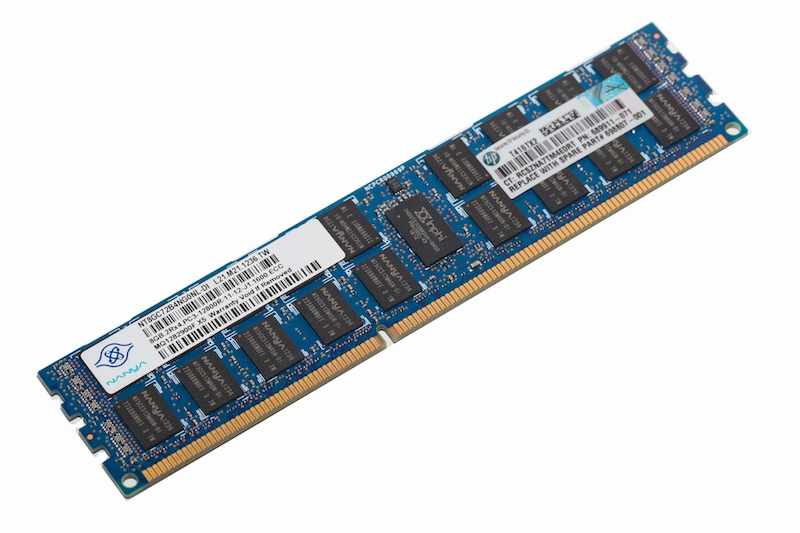
\includegraphics[width=.10\textwidth]{images/cpu-mem.jpg}};

    \node[inner sep=0pt, right=of cpu-mem] (gpu-mem)
    {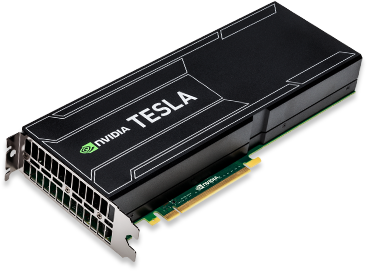
\includegraphics[width=.10\textwidth]{images/gpu-card.png}};

    \draw[*->] (CPU_device-6-2.center) -- (cpu-mem);
    \draw[*->] (GPU_device-6-2.center) -- (gpu-mem);
  \end{tikzpicture}
  \caption{\texttt{Block} and \texttt{Device\_Info} structure}
\end{figure}
\note[item]{To understand the memory synchronization, let's see the block structure}
\note[item]{Instead of directly storing pointer to memory location, another layer
  of indirection is introduced}
\note[item]{this allows support for multiple devices}
\note[item]{each device has version number}
\note[item]{whenever device updates the block, increases its version number}
\end{frame}

\begin{frame}[fragile]
  \frametitle{Block Synchronization}
  \begin{algorithmic}[1]
    \Function{Block::get\_data}{deviceid}
    \State $latest\_device \gets this.get\_latest\_device()$
    \If{$latest\_device.data\_version > this.devices[deviceid].data\_version$}
    \State {$memcpy(latest\_device.data,\ this.devices[deviceid].data)$}
    \EndIf
    \State \Return $this.devices[deviceid].data$
    \EndFunction
    % \hline
  \end{algorithmic}
\end{frame}

\begin{frame}[fragile]
  \frametitle{Optimizing Block Copy}
  \pause
  \begin{itemize}
  \item \texttt{A[i,j] = B[j,k]}
    \begin{itemize}
      \pause
    \item A is going to be read - no need to be updated
      \pause
    \item B is going to be read - update
    \end{itemize}
    \pause
  \item \texttt{C[i,j] += 2}
    \begin{itemize}
      \pause
    \item C is begin updated - update
    \end{itemize}
  \end{itemize}
\end{frame}

\begin{frame}[fragile]
  \frametitle{Memory Pinning}
  \begin{figure}[h] %place figure "here"
    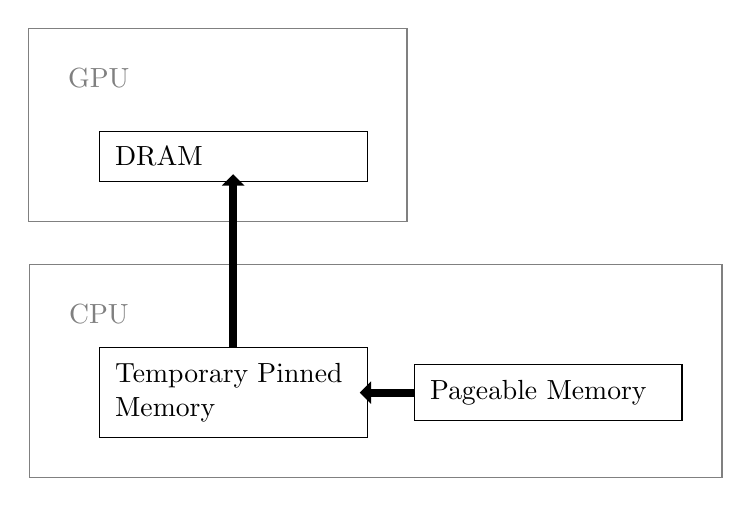
\begin{tikzpicture}[
      container/.style={draw=gray, inner sep=5mm},
      typetag/.style={draw=black, anchor=west, inner sep=2mm, text width=3cm},
      title/.style={draw=none, color=gray, inner sep=0pt}]

      \node[title]   (gpu-title)     at (0, 5) {GPU};
      \node[typetag] (gpu-ram)       at (0, 4) {DRAM};
      \node[container, fit=(gpu-title)(gpu-ram)]{};

      \pause
      \node[title]   (cpu-title)     at (0, 2) {CPU};
      \node[typetag] (pinned)        at (0, 1) {Temporary Pinned Memory};
      \node[typetag] (main-pageable) at (4, 1) {Pageable Memory};
      \node[container, fit=(cpu-title)(main-pageable)(pinned)] {};

      \pause
      \draw[draw=black, solid, line width=1mm, fill=black,
      preaction={-triangle 90, thin, draw, shorten >=-1mm}] (main-pageable) -- (pinned.east);
      \pause
      \draw[draw=black, solid, line width=1mm, fill=black,
      preaction={-triangle 90, thin, draw, shorten >=-1mm}] (pinned)        -- (gpu-ram.south);
    \end{tikzpicture}
    \caption{\texttt{memcpy} w/o memory pinning}
  \end{figure}
\end{frame}

\begin{frame}[fragile]
  \frametitle{Pinned Memory}
  \begin{figure}[h] %place figure "here"
    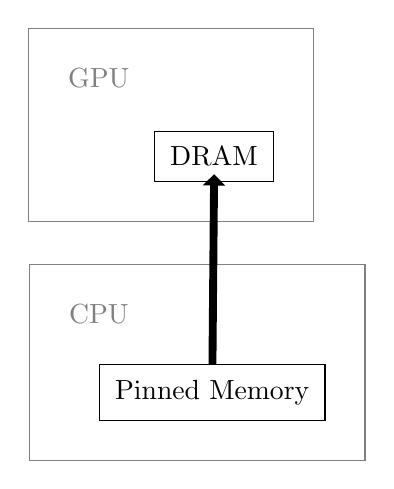
\begin{tikzpicture}[
      container/.style={draw=gray, inner sep=5mm},
      typetag/.style={draw=black, anchor=west, inner sep=2mm},
      title/.style={draw=none, color=gray, inner sep=0pt}]

      \node[title]   (gpu-title)     at (0, 5) {GPU};
      \node[typetag] (gpu-ram)       at (0.7, 4) {DRAM};
      \node[title]   (cpu-title)     at (0, 2) {CPU};
      \node[typetag] (pinned)        at (0, 1) {Pinned Memory};

      \node[container, fit=(gpu-title)(gpu-ram)] {};
      \node[container, fit=(cpu-title)(pinned)]  {};

      \pause

      \draw[draw=black, solid, line width=1mm, fill=black,
      preaction={-triangle 90, thin, draw, shorten >=-1mm}] (pinned) -- (gpu-ram.south);
    \end{tikzpicture}
    \caption{\texttt{memcpy} with memory pinning}
  \end{figure}
\end{frame}

\begin{frame}[fragile]
  \frametitle{GPU Inter Node Communication}
  \pause
\begin{figure}[h] %place figure "here"
  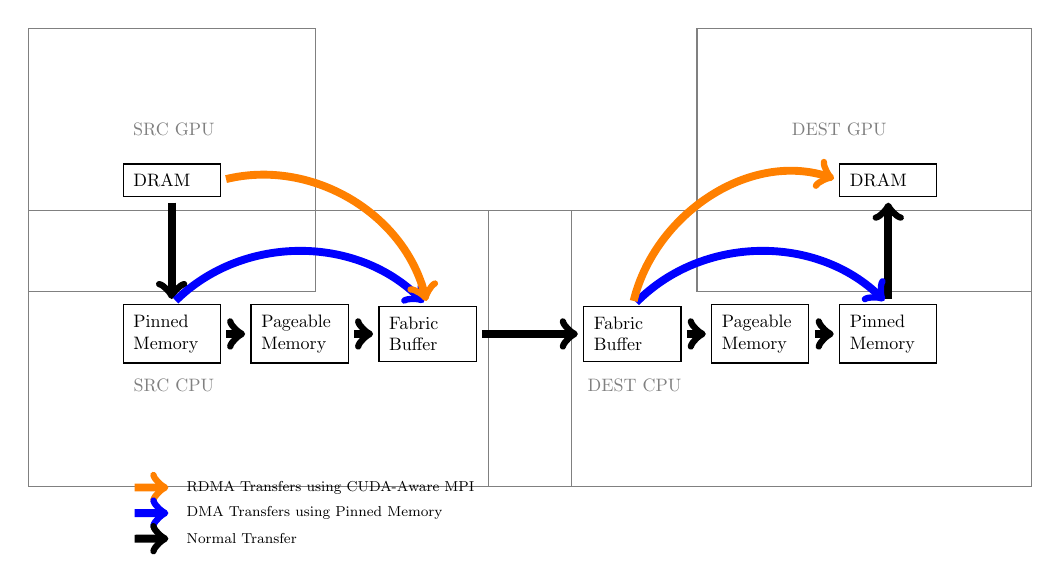
\begin{tikzpicture}[
    scale=0.65,
    every node/.style={transform shape},
    container/.style={draw=gray, inner sep=12mm},
    typetag/.style={draw=black, anchor=west, inner sep=2mm, text width=1.5cm},
    title/.style={draw=none, color=gray, inner sep=0pt},
    thickarrow/.style={->, draw=black, thick, line width=1mm, shorten <= 2pt,
      shorten >= 2pt},
    thickblue/.style={->, draw=blue, thick, line width=1mm, shorten <= 2pt,
      shorten >= 2pt, bend right=45},
    thickorange/.style={->, draw=orange, thick, line width=1mm, shorten <= 2pt,
      shorten >= 2pt, bend right=10}]

    \node[title]   (gpu-title1)     at (1, 5) {SRC GPU};
    \node[typetag] (gpu-ram1)       at (0, 4) {DRAM};
    \node[title]   (cpu-title1)     at (1, 0) {SRC CPU};
    \node[typetag] (pinned1)        at (0, 1) {Pinned Memory};
    \node[typetag] (main-pageable1) at (2.5, 1) {Pageable Memory};
    \node[typetag] (fab-buff1)      at (5, 1) {Fabric Buffer};

    \node[title]   (gpu-title2)     at (14, 5) {DEST GPU};
    \node[typetag] (fab-buff2)      at (9, 1) {Fabric Buffer};
    \node[typetag] (gpu-ram2)       at (14, 4) {DRAM};
    \node[title]   (cpu-title2)     at (10, 0) {DEST CPU};
    \node[typetag] (main-pageable2) at (11.5, 1) {Pageable Memory};
    \node[typetag] (pinned2)        at (14, 1) {Pinned Memory};

    \node[container, fit=(gpu-title1)(gpu-ram1)]                           {};
    \node[container, fit=(cpu-title1)(main-pageable1)(pinned1)(fab-buff1)] {};

    \node[container, fit=(gpu-title2)(gpu-ram2)]                           {};
    \node[container, fit=(cpu-title2)(main-pageable2)(pinned2)(fab-buff2)] {};

    \pause
    % Black arrows for src
    \draw[thickarrow] (gpu-ram1.south)      -- (pinned1.north);
    \draw[thickarrow] (pinned1.east)        -- (main-pageable1.west);
    \draw[thickarrow] (main-pageable1.east) -- (fab-buff1.west);

    \pause
    % Black arrow for network transfer
    \draw[thickarrow] (fab-buff1.east)      -- (fab-buff2.west);

    \pause
    % Black arrows for dest
    \draw[thickarrow] (fab-buff2.east)      -- (main-pageable2.west);
    \draw[thickarrow] (main-pageable2.east) -- (pinned2.west);
    \draw[thickarrow] (pinned2.north)       -- (gpu-ram2.south);

    \pause
    % Blue arrows
    \draw[thickblue] (pinned1.north) to[out=45, in=135] (fab-buff1.north);
    \draw[thickblue] (fab-buff2.north) to[out=45, in=135] (pinned2.north);

    \pause
    % Orange Arrows
    \draw[thickorange] (gpu-ram1.east) to[out=45, in=135] (fab-buff1.north);
    \draw[thickorange] (fab-buff2.north) to[out=45, in=130] (gpu-ram2.west);

    % Legend
    \node[draw=none] (l-cuda-arrow) at (0, -2) {}
      edge[thickarrow, draw=orange] (1, -2);
    \node[draw=none, text=black, right=of l-cuda-arrow] {\footnotesize RDMA Transfers using CUDA-Aware MPI};
    \node[draw=none] (l-pinned-arrow) at (0, -2.5) {}
      edge[thickarrow, draw=blue]  (1, -2.5);
    \node[draw=none, text=black, right=of l-pinned-arrow] {\footnotesize DMA Transfers using Pinned Memory};
    \node[draw=none] (l-none-arrow) at (0, -3) {}
      edge[thickarrow]  (1, -3);
    \node[draw=none, text=black, right=of l-none-arrow] {\footnotesize Normal Transfer};
    %\draw[thickarrow] (pinned1.north)   to[out=90, in=90] (fab-buff1.north);
    %\draw[thickarrow] (fab-buff2.north) to[out=90, in=90] (pinned2.north);
  \end{tikzpicture}
\end{figure}
\end{frame}

\begin{frame}[fragile]
  \frametitle{GPU Inter Node Communication}
%  \pause
%  \begin{figure}[h] %place figure "here"
%    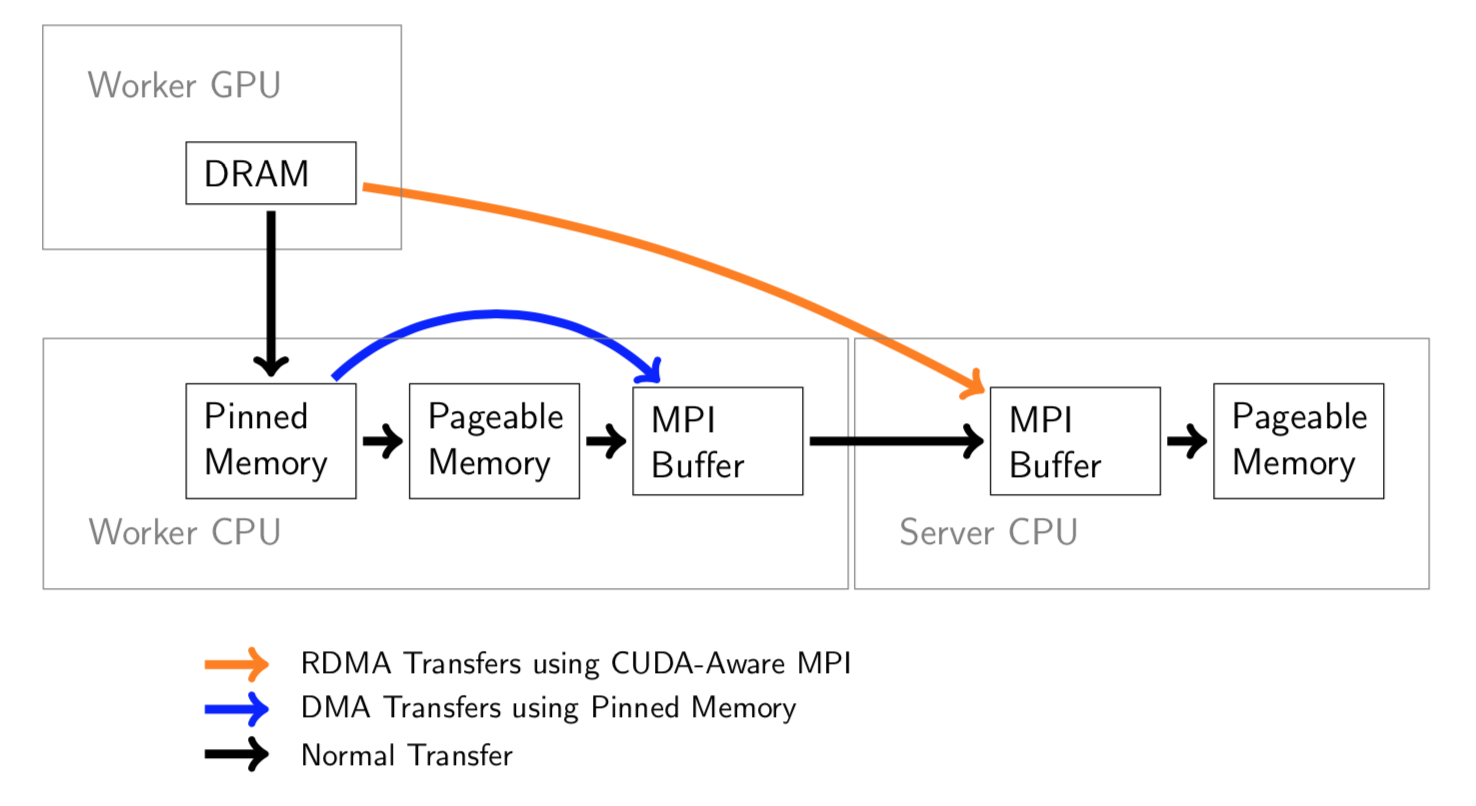
\includegraphics[width=\textwidth]{images/1gpu_comm.png}
%  \end{figure}

\begin{figure}[h] %place figure "here"
  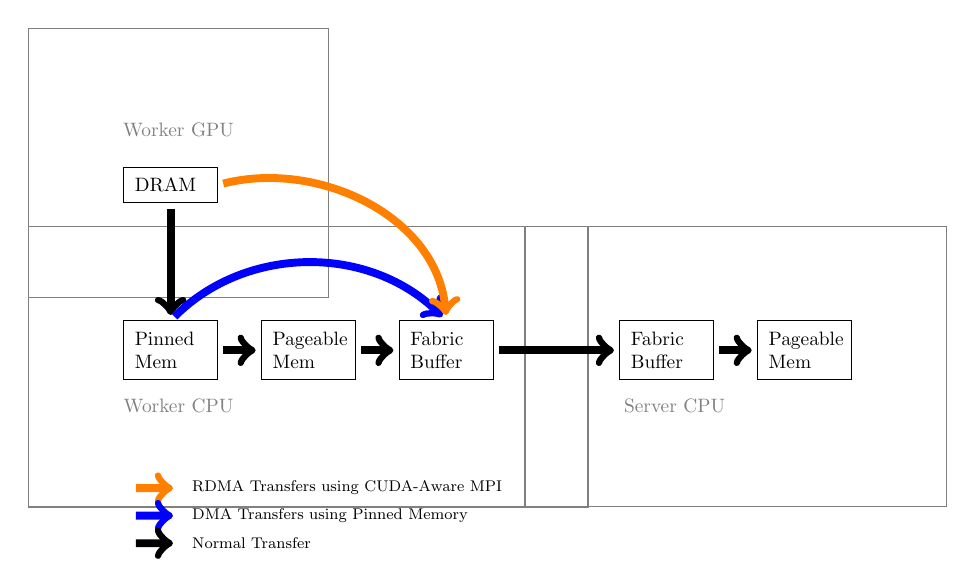
\begin{tikzpicture}[
    %transform canvas={scale=0.7},
    scale=0.7,
    every node/.style={transform shape},
    container/.style={draw=gray, inner sep=12mm},
    typetag/.style={draw=black, anchor=west, inner sep=2mm, text width=1.3cm},
    title/.style={draw=none, color=gray, inner sep=0pt},
    thickarrow/.style={->, draw=black, thick, line width=1mm, shorten <= 2pt,
      shorten >= 2pt},
    thickblue/.style={->, draw=blue, thick, line width=1mm, shorten <= 2pt,
      shorten >= 2pt, bend right=45},
    thickorange/.style={->, draw=orange, thick, line width=1mm, shorten <= 2pt,
      shorten >= 2pt, bend right=10}]

    \node[title]   (gpu-title1)     at (1, 5) {Worker GPU};
    \node[typetag] (gpu-ram1)       at (0, 4) {DRAM};
    \node[title]   (cpu-title1)     at (1, 0) {Worker CPU};
    \node[typetag] (pinned1)        at (0, 1) {Pinned Mem};
    \node[typetag] (main-pageable1) at (2.5, 1) {Pageable Mem};
    \node[typetag] (fab-buff1)      at (5, 1) {Fabric Buffer};

    \node[title]   (cpu-title2)     at (10, 0) {Server CPU};
    \node[typetag] (fab-buff2)      at (9, 1) {Fabric Buffer};
    \node[typetag] (main-pageable2) at (11.5, 1) {Pageable Mem};

    \node[container, fit=(gpu-title1)(gpu-ram1)]                           {};
    \node[container, fit=(cpu-title1)(main-pageable1)(pinned1)(fab-buff1)] {};

    \node[container, fit=(cpu-title2)(main-pageable2)(fab-buff2)] {};

    % Black arrows for worker
    \draw[thickarrow] (gpu-ram1.south)      -- (pinned1.north);
    \draw[thickarrow] (pinned1.east)        -- (main-pageable1.west);
    \draw[thickarrow] (main-pageable1.east) -- (fab-buff1.west);

    % Black arrow for network transfer
    \draw[thickarrow] (fab-buff1.east)      -- (fab-buff2.west);

    % Black arrows for dest
    \draw[thickarrow] (fab-buff2.east)      -- (main-pageable2.west);

    \pause
    % Blue arrow for fab buf
    \draw[thickblue] (pinned1.north)    to[out=45, in=135] (fab-buff1.north);
    \note[item]{Bandwidth still limited by CPU memory bandwidth}

    \pause
    % Orange arrow for fab buf
    \draw[thickorange] (gpu-ram1.east) to[out=45, in=125] (fab-buff1.north);
    \note[item]{Bandwidth of PCI-E}

    % Legend
    \node[draw=none] (l-cuda-arrow) at (0, -1.5) {}
      edge[thickarrow, draw=orange] (1, -1.5);
    \node[draw=none, text=black, right=of l-cuda-arrow] {\footnotesize RDMA Transfers using CUDA-Aware MPI};
    \node[draw=none] (l-pinned-arrow) at (0, -2) {}
      edge[thickarrow, draw=blue]  (1, -2);
    \node[draw=none, text=black, right=of l-pinned-arrow] {\footnotesize DMA Transfers using Pinned Memory};
    \node[draw=none] (l-none-arrow) at (0, -2.5) {}
      edge[thickarrow]  (1, -2.5);
    \node[draw=none, text=black, right=of l-none-arrow] {\footnotesize Normal Transfer};
    %\draw[thickarrow] (pinned1.north)   to[out=90, in=90] (fab-buff1.north);
    %\draw[thickarrow] (fab-buff2.north) to[out=90, in=90] (pinned2.north);
  \end{tikzpicture}
\end{figure}
\end{frame}

\begin{frame}[fragile]
  \frametitle{Optimized Transfer}
  \pause
  \begin{figure}[h]
    \resizebox{.9\linewidth}{!}{\input{results/optimized_block_transfer/rccsd_rhf}}
    \caption{Optimized v/s Unoptimized Block Transfers for \texttt{rccsd\_rhf.sialx}}
  \end{figure}
\end{frame}

\begin{frame}[fragile]
  \frametitle{Copy Speed}
  \pause
  \begin{figure}[h]
    \resizebox{.9\linewidth}{!}{\input{results/mempin/block_copy/pin_vs_nopin}}
    \caption{Time taken to transfer block to GPU for \textit{pinned} and \textit{non pinned} blocks}
  \end{figure}
\end{frame}

\begin{frame}[fragile]
  \frametitle{RDMA}
  \pause
  \note[item]{\texttt{GET}}
  \begin{figure}[h]
    \resizebox{.9\linewidth}{!}{\input{results/mempin/rdma/get}}
    \caption{GPU and CPU buffer passed to \texttt{GET}}
  \end{figure}
\end{frame}

\begin{frame}[fragile]
  \frametitle{RDMA}
  \pause
  \begin{figure}[h]
    \resizebox{.9\linewidth}{!}{\input{results/mempin/rdma/put}}
    \caption{GPU and CPU buffer passed to \texttt{PUT}}
  \end{figure}
\end{frame}

\begin{frame}[fragile]
  \frametitle{Overall Transfer}
  \pause
  \begin{figure}[h]
    \resizebox{.9\linewidth}{!}{\input{results/mempin/rdma/total_transfer}}
    \caption{Total MPI transfer compared to CUDA Aware MPI transfer}
  \end{figure}
\end{frame}
\begin{frame}[fragile]
  \frametitle{Memory Pinning Overhead}
  \begin{table}[h]
    \centering
    \begin{tabular}{l<{\onslide<2->} | l<{\onslide<3->} | l<{\onslide}}
      \hline
      Block Size & Pinned Memory Alloc & Non Pinned Memory Alloc \\
      \hline
      225        & 3.59733e-05         & 9.35048e-07             \\
      400        & 1.99117e-05         & 4.13507e-07             \\
      625        & 2.71294e-05         & 2.93367e-06             \\
      900        & 1.76281e-05         & 5.90459e-07             \\
      1225       & 2.44398e-05         & 6.18398e-07             \\
      1600       & 1.55177e-05         & 2.54251e-06             \\
      2025       & 2.82563e-05         & 3.18140e-06             \\
      2500       & 2.04109e-05         & 3.00072e-06             \\
      3025       & 1.91461e-05         & 3.29316e-06             \\
      \hline
    \end{tabular}
    \caption{Block Size against Page locked and non page locked memory allocation}
  \end{table}
\end{frame}

\begin{frame}[fragile]
  \frametitle{Memory Pinning Overhead}
  \note[item]{alloc}
  \begin{figure}[h]
    \resizebox{.9\linewidth}{!}{\input{results/mempin/overhead/alloc}}
    \caption{Pinned and non Pinned memory allocation}
  \end{figure}
\end{frame}

\begin{frame}[fragile]
  \frametitle{Memory Pinning Overhead}
  \begin{table}[h]
    \centering
    \begin{tabular}{l<{\onslide<2->} | l<{\onslide<3->} | l<{\onslide}}
      \hline
      Block Size & Pinned Memory Free & Non Pinned Memory Free \\
      \hline
      225        & 2.78205e-05        & 4.19095e-07            \\
      400        & 2.54586e-05        & 4.04194e-07            \\
      625        & 2.88431e-05        & 5.94184e-07            \\
      900        & 3.09199e-05        & 4.95464e-07            \\
      1225       & 2.51215e-05        & 2.44007e-07            \\
      1600       & 2.58479e-05        & 2.98023e-07            \\
      2025       & 2.80552e-05        & 3.98606e-07            \\
      2500       & 3.52804e-05        & 6.81728e-07            \\
      3025       & 2.70978e-05        & 2.64496e-07            \\
      \hline
    \end{tabular}
    \caption{Block size against Page locked and non page locked memory deallocation}
    \label{tab:mempin_free}
  \end{table}
\end{frame}

\begin{frame}[fragile]
  \frametitle{Memory Pinning Overhead}
  \note[item]{free}
  \begin{figure}[h]
    \resizebox{.9\linewidth}{!}{\input{results/mempin/overhead/free}}
    \caption{Pinned and non Pinned memory de-allocation}
  \end{figure}
\end{frame}

\begin{frame}[fragile]
  \frametitle{Caching Non Pageable Blocks}
  \begin{table}[h]
    \centering
    \begin{tabular}{l<{\onslide<2->} | r<{\onslide<3->} | r<{\onslide<4->} | r<{\onslide}}
      \hline
      File            & Not Cached & Cached     & Unpinned    \\
      \hline
      scf\_rhf\_coreh & 0.1717890  & 0.00710591 & 0.00138408  \\
      tran\_rhf\_no4v & 0.0119096  & 0.00223255 & 3.35677e-05 \\
      rccsd\_rhf      & 0.7167320  & 0.07038730 & 0.00620503  \\
      rccsdpt\_aaa    & 0.0136935  & 0.00248791 & 8.10297e-05 \\
      rccsdpt\_aab    & 0.0198253  & 0.00259629 & 4.97848e-05 \\
      \hline
    \end{tabular}
    \caption{Page Locked Cached v/s Page Locked Uncached v/s Non Page Locked allocation
      and deallocation times}
  \end{table}
\end{frame}

\begin{frame}[]
  \frametitle{Conclusion: Prefetching}
  \begin{itemize}
    \pause
  \item Prefetching makes first iteration expensive
    \pause
  \item Larger indices range can make up for it
    \pause
  \item Hit Ratio can be used as a metric to measure effectiveness of Prefetching
    \pause
  \item Prefetching helpful only when \texttt{wait\_time} is made up of network wait
    time
  \end{itemize}
\end{frame}

\begin{frame}[fragile]
  \frametitle{Conclusion: GPU}
  \begin{itemize}
    \pause
  \item GPU can speedup computation on bigger block size
    \pause
  \item Tranferring Blocks between GPU and CPU memory is expensive
    \begin{itemize}
      \pause
    \item Memory Pinning can improve the speed by invoking DMA
      \pause
      \item DMA is also invoked when transfering using MPI if memory is page locked.
    \end{itemize}
    \pause
  \item Page Locking (Memory Pinning) is expensive
    \begin{itemize}
      \pause
    \item Page Locked blocks can be cached
      \pause
    \item SIA blocks usage is predictable, effective caching algorithm can be devised
    \end{itemize}
  \end{itemize}
\end{frame}

\end{document}
